% title: Human review belongs to the walk runner
% description: At a tagged review point, the runner passes the equation output to human review, then sends the accepted or edited value into the walk generator before the next equation runs.
\documentclass[tikz,border=5pt]{standalone}
\usetikzlibrary{arrows.meta,calc,shapes.geometric}
\definecolor{numeric}{HTML}{4477AA}
\definecolor{textual}{HTML}{AA4499}

\tikzset{
    box/.style={draw, line width=0.8pt, minimum height=0.8cm,
                minimum width=1.8cm, inner sep=6pt, align=center},
    ir/.style={box},
    flow/.style={-{Stealth[length=5pt]}, line width=0.9pt},
    feedback/.style={flow, dashed},
    note/.style={font=\small, align=center},
    choice/.style={diamond, draw, line width=0.8pt,
                   aspect=2, inner sep=2pt, align=center},
}

\newcommand{\irframe}[2]{
    \draw[line width=0.8pt] #1 rectangle #2;
}

\newcommand{\transformarrow}[4][above]{
    \draw[flow] (#2) -- node[#1=6pt,note] {#4} (#3);
}

\begin{document}
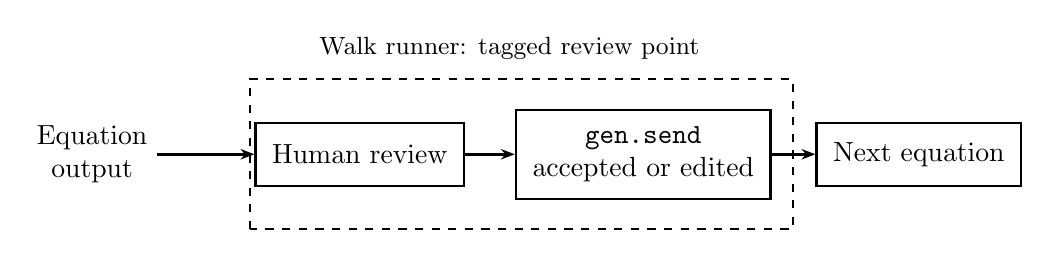
\begin{tikzpicture}

    \node[align=center] (out) at (0,0) {Equation\\output};
    \node[box] (review) at (3.4,0) {Human review};
    \node[box] (send) at (7,0) {\texttt{gen.send}\\accepted or edited};
    \node[box] (next) at (10.5,0) {Next equation};
    \draw[flow] (out) -- (review);
    \draw[flow] (review) -- (send);
    \draw[flow] (send) -- (next);
    \draw[dashed,line width=0.7pt] (2,-0.95) rectangle (8.9,0.95);
    \node[note] at (5.3,1.35) {Walk runner: tagged review point};

\end{tikzpicture}
\end{document}
